\documentclass[a4paper]{article}
\usepackage{fullpage}
\usepackage[scaled]{helvet}

% Fix \paragraph to have a newline
\makeatletter
\renewcommand\paragraph{\@startsection{paragraph}{4}{\z@}%
  {-3.25ex\@plus -1ex \@minus -.2ex}%
  {1.5ex \@plus .2ex}%
  {\normalfont\normalsize\bfseries}}
\makeatother

\setcounter{secnumdepth}{4}	% Number \paragraphs

\renewcommand\maketitle{
%\ifpdf
\pdfinfo{
   /Author (\getauthor)
   /Title  (\getprojectname  - \gettitle)
   /Producer (John Hodge)
}
%\fi


\begin{titlepage}

\begin{center}

\vspace{1cm}

\textsc{\LARGE \getprojectname}\\[0.5cm]
\textsc{\huge \gettitle}\\[0.5cm]
\rule{0.9\textwidth}{0.7pt} \\[0.75cm]
% Authors
\emph{\getauthor} \\[0.5cm]
% Client
Client: \emph{\getclient} \\[0.5cm]

CITS3200 Professional Computing 2011 \\
University of Western Australia Crawley, WA, 6009

\vspace{2cm}
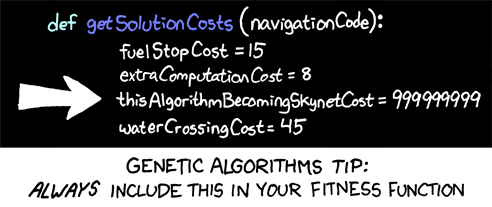
\includegraphics{../534-genetic_algorithms.png} \\
\centering{\footnotesize XKCD \#534 - Genetic Algorithms - CC BY-NC 2.5}

\end{center}

\end{titlepage}
}

\def\csharp{\ensuremath{C\sharp } }

\def\getprojectname{}
\def\projectname#1{\gdef\getprojectname{#1}}
\def\getclient{}
\def\client#1{\gdef\getclient{#1}}
\makeatletter
\newcommand\gettitle{\@title}
\newcommand\getauthor{\@author}
\makeatother

\projectname{Genetic Engine Project}
\title{Requirements Analysis Document}
\author{Rohit Gopalan, John Hodge, Alwyn Kyi, Brian Marshall, Antriksh Srivastava}
\client{Mr Peter Th\"ornell}

\begin{document}

\maketitle

\tableofcontents

\clearpage

\paragraph*{Revision History}
\begin{itemize}
\item Version R0.1 08/08/2011 R Gopalan. Created
\item Version R0.2 24/Aug/2011 J Hodge. Converted to tex
\end{itemize}

\subsection*{Preface}
This document addresses the requirements of the Genetic Engine system. The intended audience for this document are the designers and the client of the project.

\paragraph*{Target Audience}
Client, Developers

\paragraph*{Meeting Times (Past and upcoming times)}
\begin{itemize}
\item Group Meeting was held on 08/08/2011, 10am at Hacket Hall Café, University of Western Australia
\item Client Meeting was held on 08/08/2011, 11am at Hacket Hall Café, University of Western Australia
\item Group Meeting was held on 15/08/2011, 1pm at Lab 2.01 in CSSE School, UWA
\item Client Meetng was held on 17/08/2011, 2pm at Reid Library, UWA
\item Group Meeting to be held on 22/08/2011, 11am at Hacket Hall Cafe, UWA
\item Client Meeting to be held on 24/08/2011, 2pm at Reid Library, UWA
\end{itemize}

\paragraph*{Milestones}
26/08/2011 RAD Part 1 (Deliverable A) Due

\paragraph*{Client Sign-off}

\clearpage


%
% General Goals
%
\section{General Goals}
The aim of the system is to provide a general implementation of a genetic algorithm. 
This will be done by providing an API through the .Net library in \csharp. 
% For this section, enter the goals of your subsystem, i.e. what are the objectives of the functions of your subsystem?


%
% Current System
%
\section{Current System}
There is no current system. % *waves hand*
This software is not replacing a current implementation, or being used to suppliment known techniques (at least in the client's case).
%For this section, describe the current situation that is relevant to your subsystem.


%
% Proposed System
%

\section{Proposed System}
\subsection{Overview}
The Genetic Engine will provide a general implementation of a genetic algorithm. It will configurable and extensible to run a variety of specific genetic algorithms.
An example implementation of a genetic algorithm is also required. This will accept a map with the locations of towns and the start and end points of a path. It will generate a path which balances two requirements. These requirements are to minimize the total path length and to minimize the distance of each town from its closest point on the path. This will include a tool to visualise individual paths generated by the algorithm.

\subsection{Functional Requirements}
\paragraph*{Core .Net Library (DLL) written in \csharp exposing}
\begin{itemize}
 \item Genetic engine class
 \begin{itemize}
  \item Maximum flexibility
  \item Accept arbitrary class as chromosome.
  \item Configurable via plug-ins for initial population, fitness function, genetic operators and termination condition.
  \item Write the best individuals of each generation to a file.
 \end{itemize}
 \item Plug-in Loader
 \begin{itemize}
  \item Load plug-in classes from user-specified .Net DLL files.
  \item Create instances of plug-in classes for use in the genetic engine.
 \end{itemize}
\end{itemize}

\paragraph*{Support .Net Library (DLL) written in \csharp exposing}
\begin{itemize}
 \item Interfaces to be implemented by plug-in classes
 \item Other classes required by plug-in classes
\end{itemize}

\paragraph*{Command-line application written in \csharp}
\begin{itemize}
 \item Reads XML configuration file identifying the plug-ins and other parameters to run the algorithm with.
 \item Loads plug-ins from .Net DLL files.
 \item Runs the genetic engine with the selected plug-ins and parameters.
\end{itemize}

\paragraph*{Sample plug-ins and configuration files for the path optimisation problem}
\begin{itemize}
 \item{Chromosome Generator}: Loads map file and generates random paths in the map:
 \item{Fitness function}: Assigns higher fitness to paths which are shorter and approach closer to the cities.
 \item{Genetic operators}
 \begin{itemize}
  \item 2 Path mutation operators 
  \item 2 Path conjugation operators
 \end{itemize}
 \item Terminator
\end{itemize}

\paragraph*{Visualisation Application}
\begin{itemize}
 \item Load paths from text file outputted by genetic engine when run with example plug-ins.
 \item Display the path on its map.
\end{itemize}

\paragraph{Note}
Paths will be in the form of trees. That is, each path will be an undirected graph which is connected and has no cycles. For simplicity, the vertices in the tree (not the edges) will be used when determining the minimum distance of the path from each town.

An undirected graph would have been a more general representation of the path however, any graph can be reduced to a tree by removing edges. The resulting tree will contain all the same vertices, remain connected and have total length less than or equal to the original graph. This simplifies the algorithm as it is much easier to define conjugation operations for trees than for graphs.


\subsection{}
\subsubsection{User Interface and Human Factors}
The users of the genetic engine, sample plug-ins and visualiser tool will be programmers with some experience with \csharp. Therefore, clear API and source code documentation are the most important source of information.

The sample plug-ins have little practical value in themself other than proof that the genetic engine library works. However, their source code will serve as an example of how to utilise the classes within the library.

\subsubsection{Documentation}
\paragraph{Core genetic engine library and support library}
\begin{itemize}
 \item API documentation outlining all exposed classes and how they are intended to be used.
 \item Tutorial document with step-by-step instructions for a simple example application using the library.
 \item Clear and complete source code documentation.
\end{itemize}

\paragraph{Command-line application}
\begin{itemize}
 \item Explanation of all command line options with examples
 \item Explanation of XML configuration file format with examples
\end{itemize}

\paragraph{Sample Plug-ins and Visualisation Tool}
\begin{itemize}
 \item Usage instructions
 \item Clear and complete source code documentation.
\end{itemize}

\subsubsection{Hardware Consideration}
The libraries and applications should work on any machine capable of running .Net. Although faster hardware will obviously result in faster solutions.

\subsubsection{Performance Characteristics}
Performance has a lower priority than flexibility and good object oriented code structure however where possible, without sacrificing these, optimisations for speed should be made.

\subsubsection{Error Handling and Extreme Conditions}
The classes in the genetic engine libraries should throw clear and descriptive exceptions when its methods are called incorrectly. These should assist the programmer using these libraries to quickly identify and fix their errors.

The command-line application should identify problems with the configuration as early as possible and report it in a clear format, identifying the items which caused the problem and explaining why they are invalid. It should also capture the exceptions thrown by the genetic engine library classes and report them in an easy to read format, indicating the plug-in which caused the problem.

\subsubsection{System Interfacing}
The only I/O actually required is the parameters (through the use of plugin files) that are fed into the engine in the beginning. These parameters can be set through an API but may also implement a command line interface and a GUI. After those parameters are set, the program will run its course through a number of iterations.

The output will be set by a visualization plugin if it is implemented in the future, otherwise the data will be saved to a text file.

\subsubsection{Quality Issues}
The highest priority of the Genetic Engine is its flexbility so it should be able to handle any type of compatible plugin that is fed into it without errors. Error checking will be implemented to check that the plugins are in fact compatible with the engine and written correctly. 
% For this section, focus on the possible quality enhancement or compromises. Consider the following: 
% What are the requirements for reliability? Must the system trap faults? Is there a maximum acceptable time for restarting the system after a failure? What is the acceptable system downtime per 24-hour period? Is it important that the system be portable (able to move to different hardware or operating system environments)? 

\subsubsection{System Modifications}
There is a set specification as to what the underlying engine should do, only minor modifications can be made and only at a higher level (client interface). This includes things such as how the engine accepts input, rather than how it processes it.
% For this section, think about the current infrastructure of your system which will be extended for future features, incorporated or made obsolete. Consider the following: 
% What parts of the system are likely candidates for later modification? What sorts of modifications are expected? 

\subsubsection{Physical Environment}
The Genetic Engine will run on a regular computer so no extreme physical conditions will be present.
% For this section, consider the physical environment in which your subsystem will exist. Consider the following: 
% Where will the target equipment operate? Will the target equipment be in one or several locations? Will the environmental conditions in any way be out of the ordinary (for example, unusual temperatures, vibrations, magnetic fields ...)?

\subsubsection{Security Issues}
There are no real security issues with the system however the engine will be encapsulated to ensure that the user does not modify the internal program data and risk a malfunction.

\subsubsection{Resource Issues}
% Antkrish - Not sure what to put here
The engine deals with a set of plugins upon which it will iterate through generations, and then output this to a file. The user is responsible for this file once it has been created. 

The engine will be self-sustaining and does not really require installation though the user will need to know how to specify plugins.
% For this section, think about data management for your subsystem. Consider the following: 
% How often will the system be backed up? Who will be responsible for the back up? Who is responsible for system installation? Who will be responsible for system maintenance? 

\subsection{Constraints}
The project is to be developed in \csharp using Visual Studio or MonoDevelop.
\subsection{System Model}
% You will have to use the UML (Unified Modelling Language) to create the models. If the CASE tools is not installed yet (Together-J), you can use Visio or PowerPoint to produce the models. For more information on the notations of UML, check out the following Rational websites - Notation and Documentation. To make your models more readable, you have to include some texts to guide the reader along the flow of your model. These text are called Navigational Text because they help to move the reader along the models.

\subsubsection{Scenarios}
The engine must be programmed in \csharp as specified by the client. It will be developed in Microsoft Visual Studio. It will itself be a library (.dll) and should be compatible with modern systems.
% For this section, think about all the possible ways which the users will interact with your subsystem. Present them in a "story" format.

\subsubsection{Use Case Models}
TODO
\paragraph{Actors}
\paragraph{Use Cases}

\subsubsection{Object Models}
TODO
\paragraph{Data Dictionary}
\paragraph{Class Diagrams}

\subsubsection{Dynamic Models}
TODO
\subsubsection{User Interface - Navigational Paths and Screen Mockups}

Figure 3.1 The screen mock-up of the Genetic Engine Interface. Each plugin is to be specified by their file-path.
% TODO: Include figure

Figure 3.2 Pathfinding using Genetic Algorithms shown visually in Gridview 
% TODO: Include figure

%
% Glossary
%
\section{Glossary}

\end{document}

